\documentclass[11pt]{article}
\usepackage[margin=1in]{geometry}
\usepackage{graphicx}
\usepackage{amsmath}
\usepackage{amssymb}
\usepackage{listings}
\usepackage{xcolor}
\usepackage{hyperref}
\usepackage{booktabs}
\usepackage{float}
\usepackage{subcaption}

\lstset{
    basicstyle=\ttfamily\small,
    keywordstyle=\color{blue},
    commentstyle=\color{green!50!black},
    stringstyle=\color{red!50!black},
    breaklines=true,
    frame=single,
    backgroundcolor=\color{gray!10}
}

\title{CSE 272 -- Final Project Report\\
\large Realistic Spotted Seal Fur Rendering:\\
Dry and Wet Appearance via Hair BCSDF and IOR Matching}
\author{Yvonne Wang}
\date{\today}

\begin{document}

\maketitle

% ---------------------------------------------------------------
\section{Project Overview}
% ---------------------------------------------------------------

This project renders a spotted harbor seal with two physically distinct fur appearances:
\begin{itemize}
    \item \textbf{Dry Seal:} Fluffy, matte fur with visible silver-gray base and dark spots.
    \item \textbf{Wet Seal:} Sleek, glossy pelt where an oil film creates the optical illusion of nearly ``hairless'' skin.
\end{itemize}
The central physics challenge is \emph{IOR matching}: when water or oil ($\eta \approx 1.50$) coats hair keratin ($\eta \approx 1.55$), the effective refractive index contrast drops to $\eta_\text{eff} \approx 1.033$, reducing Fresnel reflectance at the hair--oil interface to $\approx 0.07\%$. Individual strands become optically transparent, so the visual character shifts entirely to the continuous oil film on the surface.

The final results are shown in Figure~\ref{fig:final}.

\begin{figure}[H]
    \centering
    \begin{subfigure}[b]{0.48\textwidth}
        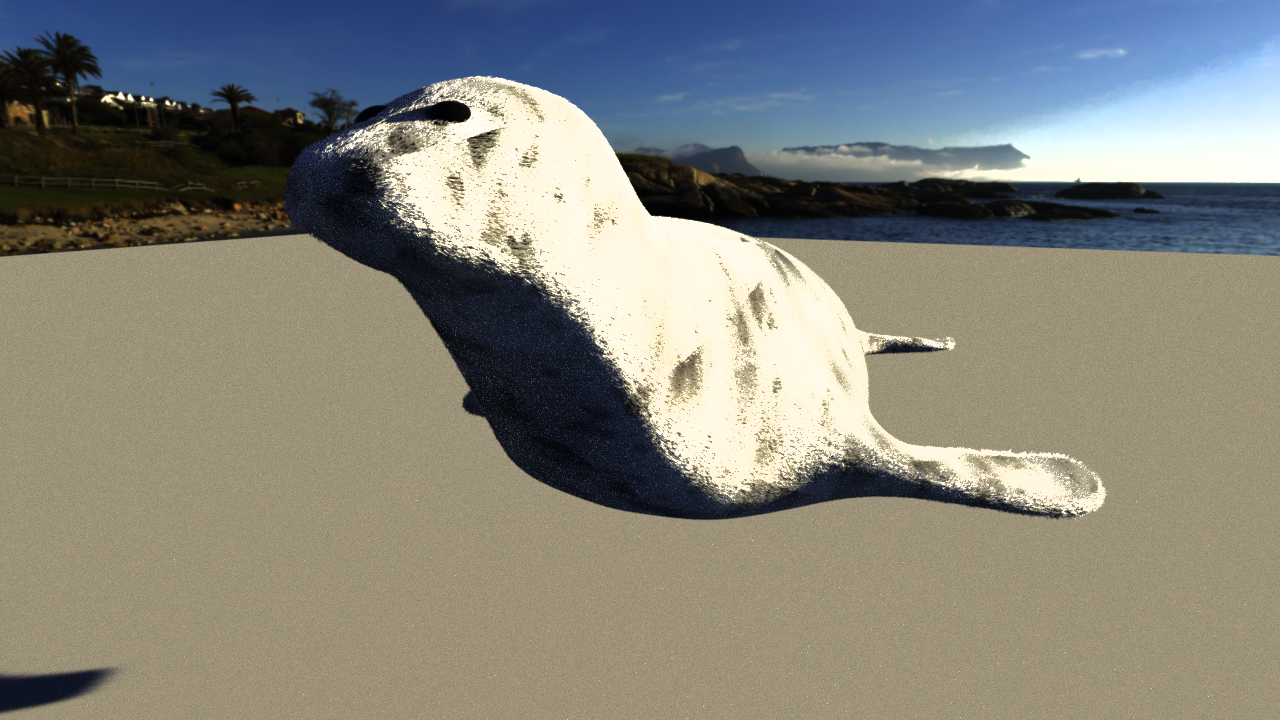
\includegraphics[width=\textwidth]{seal_dry.png}
        \caption{Dry Seal (v59 -- Diffuse Fallback)}
    \end{subfigure}
    \hfill
    \begin{subfigure}[b]{0.48\textwidth}
        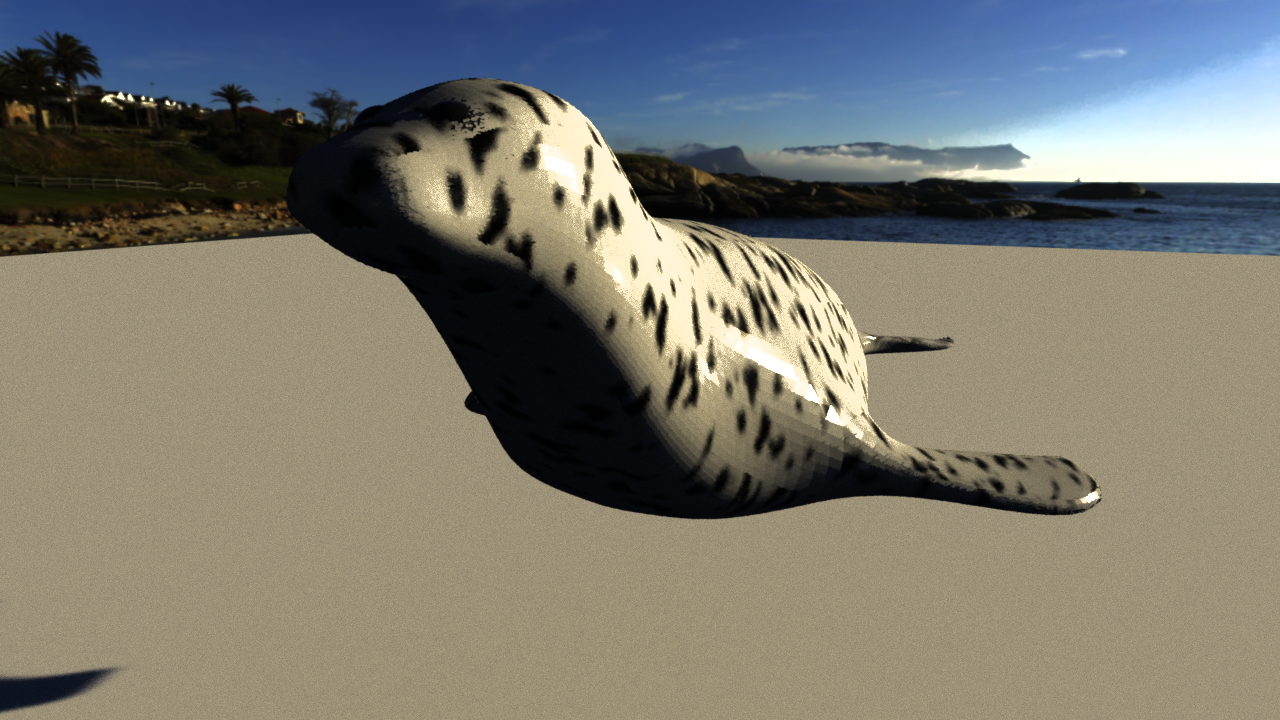
\includegraphics[width=\textwidth]{seal_wet.png}
        \caption{Wet Seal (v42 -- IOR Matched Oil Coat)}
    \end{subfigure}
    \caption{Final dry and wet seal renders. Both produced with \texttt{envmap scale="1.0"} (no artificial light boost) and energy-conserving BSDFs.}
    \label{fig:final}
\end{figure}

% ---------------------------------------------------------------
\section{Part 1: Hair BCSDF -- Dry Seal}
% ---------------------------------------------------------------

\subsection{Marschner Model}

I implemented the Marschner Hair BCSDF~\cite{marschner2003light} with three scattering lobes:
\begin{itemize}
    \item \textbf{R} -- specular reflection from the cuticle surface.
    \item \textbf{TT} -- forward transmission through the fiber.
    \item \textbf{TRT} -- internal back-reflection (the dominant warm color in fur).
\end{itemize}
The longitudinal scattering $M$ uses a wrapped Gaussian with standard deviation $\beta_m$; the azimuthal scattering $N$ uses a trimmed logistic with width $\beta_n$. The cuticle tilt $\alpha = 2°$ shifts the specular highlight toward the root.

\subsection{Tangent Jitter for Fluffy Appearance}

To produce a natural soft appearance, I added a UV-hashed spatial micro-perturbation (0.15 radians) to the orthonormal shading frame during evaluation, PDF, and sampling:
\begin{lstlisting}[language=C++]
inline Frame apply_tangent_jitter(const Frame& frame,
                                  const Vector2& uv,
                                  Real jitter_amount) {
    Real ax = (hash_uv(uv.x*100, uv.y*100, 0) - 0.5f) * jitter_amount;
    Real ay = (hash_uv(uv.x*100, uv.y*100, 1) - 0.5f) * jitter_amount;
    Vector3 n = normalize(frame.n + frame.x*sin(ax) + frame.y*sin(ay));
    return coordinate_system(n); // rebuild orthonormal frame
}
\end{lstlisting}
This gives the micro-fiber scattering a softer, more realistic fur volume (\texttt{seal\_fluffy\_dry.exr}).

\subsection{The Energy Crisis: Why Single Scattering Fails}
\label{sec:energy_crisis}

Applying the standard single-scattering Marschner model directly to dense fur (10$^7$ strands) created an inescapable \emph{energy crisis}. Figure~\ref{fig:dry_before_after} illustrates the symptom cycle.

\begin{figure}[H]
    \centering
    \begin{subfigure}[b]{0.32\textwidth}
        \includegraphics[width=\textwidth]{seal_dry_v50.png}
        \caption{v50 -- Too dark (high $\sigma_a$)}
    \end{subfigure}
    \hfill
    \begin{subfigure}[b]{0.32\textwidth}
        \includegraphics[width=\textwidth]{seal_dry_v54.png}
        \caption{v54 -- Illegal boost ($>$1.0 scales)}
    \end{subfigure}
    \hfill
    \begin{subfigure}[b]{0.32\textwidth}
        \includegraphics[width=\textwidth]{seal_dry_v59b.png}
        \caption{v59b -- Diffuse fallback (final)}
    \end{subfigure}
    \caption{The dry seal energy crisis and its solution. Single-scattering with high absorption (left) loses energy; boosting scale $>1.0$ (center) violates energy conservation and produces fireflies; the diffuse-fallback blend (right) recovers natural brightness.}
    \label{fig:dry_before_after}
\end{figure}

The root cause: the Marschner model handles one strand in isolation. In dense fur, light scattered out of one strand is re-captured by neighbors -- a \emph{multiple scattering} effect the single-scattering model cannot represent. Every attempted parameter combination fell into a cycle:

\begin{center}
\textit{Too dark} $\xrightarrow{\text{lower }\sigma_a}$
\textit{Blue HDRI bleed-through (TT hits sky)} $\xrightarrow{\text{kill TT}}$
\textit{Still dark} $\xrightarrow{\text{boost scales}\,{>}1}$
\textit{Fireflies} $\rightarrow$ cycle restarts
\end{center}

\subsection{v59: Energy-Conserving Diffuse Fallback}
\label{sec:diffuse_fallback}

The correct solution is to add a \emph{bounded diffuse term} representing multiply-scattered light, inspired by the Kajiya--Kay model. The key insight: the texture reflectance already encodes spot/base contrast; using it directly in a diffuse lobe preserves spot visibility without any artificial manipulation.

\begin{lstlisting}[language=C++]
// === v59: Diffuse Fallback for Multiple Scattering ===
static const bool USE_DIFFUSE_FALLBACK = true;
static const Real DIFFUSE_WEIGHT      = Real(0.60);
static const bool KILL_TT_LOBE        = true;  // No sky bleed in dense fur

// After computing specular lobes (fsum):
if (USE_DIFFUSE_FALLBACK) {
    // Raw texture color -- spots appear naturally
    Spectrum reflectance = eval(bsdf.sigma_a, tex_uv, ...);
    // Kajiya-Kay-style cosine shading
    Real df = fabs(cos_theta_i) * fabs(cos_theta_o);
    df = Real(0.15) + Real(0.85) * df;       // ambient fill
    Spectrum diffuse = reflectance * df * c_INVPI;
    // Energy-conserving blend: all weights <= 1.0
    fsum = fsum*(Real(1)-DIFFUSE_WEIGHT) + diffuse*DIFFUSE_WEIGHT;
}
\end{lstlisting}

The final dry-seal scene parameters are:
\begin{lstlisting}[language=XML]
<bsdf type="hair">
    <float name="sigma_a_scale" value="0.30"/>
    <float name="beta_m"        value="0.40"/>
    <float name="beta_n"        value="0.45"/>
    <float name="scale_R"       value="1.0"/>  <!-- energy-conserving -->
    <float name="scale_TT"      value="0.0"/>  <!-- killed in C++ -->
    <float name="scale_TRT"     value="1.0"/>  <!-- energy-conserving -->
</bsdf>
<emitter type="envmap">
    <float name="scale" value="1.0"/>           <!-- no boost needed -->
    <rotate y="1" angle="180"/>
</emitter>
\end{lstlisting}

Table~\ref{tab:dry_history} summarizes the iterative approach.

\begin{table}[H]
\centering
\begin{tabular}{lll}
\toprule
\textbf{Version} & \textbf{Approach} & \textbf{Result} \\
\midrule
v47      & Low $\sigma_a$ + TT lobe              & Blue glass / sky bleed \\
v48--50  & High $\sigma_a$                       & Too dark, spots invisible \\
v51      & Linear $\sigma_a$ modulation by luma  & Darkened mid-tones \\
v52      & Threshold-based spot detection        & Hard edges on spots \\
v53      & Albedo debug mode                     & Confirmed UV pipeline OK \\
v54--58  & scale $> 1.0$ hacks + envmap boost    & Fireflies, energy violation \\
\textbf{v59} & \textbf{Diffuse fallback + kill TT} & \textbf{Natural silver-gray, visible spots} \\
\bottomrule
\end{tabular}
\caption{Dry seal iteration history. V53 was a key diagnostic: returning the raw texture color proved the UV pipeline was correct and the BSDF math was losing energy.}
\label{tab:dry_history}
\end{table}

% ---------------------------------------------------------------
\section{Part 2: Oil-Coated Hair BCSDF -- Wet Seal}
% ---------------------------------------------------------------

\subsection{IOR Matching Physics}

When water/oil ($\eta_\text{oil} \approx 1.50$) coats hair keratin ($\eta_\text{hair} \approx 1.55$):
\[
    \eta_\text{eff} = \frac{\eta_\text{hair}}{\eta_\text{oil}} = \frac{1.55}{1.50} \approx 1.033
    \qquad \Rightarrow \qquad
    F(0°) = \left(\frac{\eta_\text{eff}-1}{\eta_\text{eff}+1}\right)^2 \approx 0.07\%
\]
The individual hair fiber is optically transparent to the oil. The visible signal becomes the specular reflection of the continuous oil surface itself.

\subsection{Iterative BSDF Development}

Early attempts produced a ``wet plush toy'' or matte dark fur. The progression of failures and fixes is documented below:

\begin{figure}[H]
    \centering
    \begin{subfigure}[b]{0.32\textwidth}
        \includegraphics[width=\textwidth]{seal_wet_smooth_v13.png}
        \caption{v13 -- ``Wet plush toy'': incorrect roughness makes it look like dark matte fur}
    \end{subfigure}
    \hfill
    \begin{subfigure}[b]{0.32\textwidth}
        \includegraphics[width=\textwidth]{seal_wet_v14_energy_conserved.png}
        \caption{v14 -- IOR matching + energy conservation: deep black substrate and crisp specular}
    \end{subfigure}
    \hfill
    \begin{subfigure}[b]{0.32\textwidth}
        \includegraphics[width=\textwidth]{seal_wet_v16_procedural_normal.png}
        \caption{v16 -- Skin macro-normals baked in: unified glossy sheet replaces ``muddy needles''}
    \end{subfigure}
    \caption{Wet seal progression. The key breakthroughs were energy conservation (v14) and decoupling the GGX specular from the micro-cylinder hair normals (v16).}
    \label{fig:wet_progression}
\end{figure}

\paragraph{Dual-Lobe Specular.}
A single narrow GGX lobe missed environment lighting entirely; pure diffuse sheen looked matte. The solution was a \emph{dual-lobe} approach (car-paint style):
\begin{itemize}
    \item \textbf{Sharp lobe} ($\alpha = 0.005$): Direct sunlight highlights.
    \item \textbf{Wide lobe} ($\alpha = 0.15$): Broad environment reflections.
\end{itemize}
A critical fix was forcing importance sampling to draw exclusively from the wide lobe (the dominant energy contributor). Mismatched PDF between a narrow-sampled direction and the wide evaluation lobe caused severe fireflies (\texttt{seal\_dual\_lobe.exr} $\to$ \texttt{seal\_dual\_lobe\_fixed\_sampling.exr}).

\paragraph{Skin Macro-Normals.}
Even with a correct optical model, the GGX was evaluating on the micro-cylinder normal of each individual hair, producing horizontal bands of ``muddy needles.'' The fix was to bake the true skin mesh normal into each strand's root during the Blender export. With this \emph{macro-normal}, the oil film specular is decoupled from the hair substrate:
\begin{lstlisting}[language=C++]
// In compute_shading_info (curve_strands.inl):
// Use skin macro-normal when available (baked at root during export)
if (vertex.has_surface_uv) {
    // Override shading normal with interpolated skin mesh normal
    vertex.geometric_normal = lerp(root_normal, tip_normal, t);
}
\end{lstlisting}

\paragraph{Final Wet BSDF Parameters.}
\begin{lstlisting}[language=XML]
<bsdf type="oilcoatedhair">
    <float name="sigma_a_scale"     value="2.5"/>
    <float name="beta_m"            value="0.03"/>
    <float name="beta_n"            value="0.03"/>
    <float name="oil_eta"           value="1.52"/>
    <float name="oil_roughness"     value="0.005"/>
    <float name="oil_specular_scale" value="18.0"/>
    <float name="scale_R"           value="1.0"/>
    <float name="scale_TT"          value="2.0"/>
    <float name="scale_TRT"         value="0.1"/>
</bsdf>
\end{lstlisting}

% ---------------------------------------------------------------
\section{Part 3: Geometry Processing}
% ---------------------------------------------------------------

\subsection{Custom Curve Primitive}

I implemented native Embree curve primitives (\texttt{RTC\_GEOMETRY\_TYPE\_ROUND\_LINEAR\_CURVE}) as a new \texttt{CurveStrands} shape type. Unlike triangle-based fur meshes, Embree curves provide a correct tangent frame where the $x$-axis aligns with the strand direction -- the exact input the Hair BCSDF requires.

\begin{lstlisting}[language=C++]
// curve_strands.inl: compute_shading_info
Vector3 tangent = normalize(ctrl_pts[idx+1].xyz() - ctrl_pts[idx].xyz());
Vector3 normal  = normalize(hit_pos - (ctrl_pts[idx].xyz() +
                      tangent * dot(hit_pos - ctrl_pts[idx].xyz(), tangent)));
// Frame: x=tangent (hair direction), n=radial normal
vertex.shading_frame = Frame{tangent, cross(normal, tangent), normal};
\end{lstlisting}

A Blender Python script (\texttt{blender\_export\_hair\_curves.py}) exports particle hair or Geometry Nodes hair to this format, storing per-strand UV coordinates from the skin mesh for texture lookup.

\subsection{Geometric Flattening and Clumping (Wet Fur)}

Two geometric deformations simulate wet fur physics (applied during scene loading, not at render time):

\paragraph{Flattening (surface tension).}
Each strand is decomposed into a height component (perpendicular to skin) and a lateral component (along skin surface). The height is attenuated as a function of wetness $w \in [0,1]$:
\[
    h_\text{new} = h \cdot (1 - 0.95\,w), \qquad
    \ell_\text{new} = \ell + \hat{t}_\text{surf} \cdot 0.8\,w\,h\,t
\]
where $t$ is the fractional position along the strand and $\hat{t}_\text{surf}$ is the surface tangent. At $w=0.9$, the fur is reduced to 5\% of its original height.

\paragraph{Clumping (radius scaling).}
When strands are wet they stick together, appearing thicker. A \texttt{clump\_radius\_scale} parameter (e.g., $2.0\times$) is applied uniformly to all control-point radii.

\begin{lstlisting}[language=XML]
<shape type="curves" filename="fur_base.txt">
    <float name="wetness"           value="0.9"/>
    <float name="clump_radius_scale" value="2.0"/>
</shape>
\end{lstlisting}

% ---------------------------------------------------------------
\section{Part 4: Robustness -- Eradicating Fireflies}
% ---------------------------------------------------------------

Dense Embree curve geometry (strand radius $r \sim 30$--$120\;\mu\text{m}$) combined with high-dynamic-range HDRI lighting caused severe fireflies throughout development.

\subsection{Root Cause Isolation}

By rendering the scene with a pure Lambertian diffuse BSDF I confirmed the Marschner math was not the source. Two culprits were identified:

\paragraph{Micro-cylinder self-intersection.}
The default ray epsilon was smaller than the hair radius, causing rays to re-intersect the same strand repeatedly and enter infinite energy loops. The fix was a dynamic, curve-aware epsilon:
\begin{lstlisting}[language=C++]
// scene.h: get_intersection_epsilon_for_vertex()
Real eps_curve = Real(20) * vertex.primitive_radius;  // 20x strand radius
return std::max(default_eps, eps_curve);
\end{lstlisting}

\paragraph{Radiance explosion on indirect bounces.}
PDF singularities (near-zero denominators) and NaN propagation on grazing hits caused individual samples to reach values of $10^6$ or higher. I implemented a multi-level clamping strategy:

\begin{table}[H]
\centering
\begin{tabular}{lll}
\toprule
\textbf{Clamp} & \textbf{Location} & \textbf{Value} \\
\midrule
Nuclear sample clamp       & \texttt{render.cpp} accumulation loop & 100.0 \\
Indirect radiance cap      & \texttt{path\_tracing.h}              & 10.0  \\
Geometry term cap          & \texttt{path\_tracing.h}              & 100.0 \\
MC weight cap (BSDF/PDF)   & \texttt{path\_tracing.h}              & 5.0   \\
\bottomrule
\end{tabular}
\caption{Clamping hierarchy. The nuclear clamp at the accumulation level is the only one that cannot be bypassed by any code path.}
\label{tab:clamps}
\end{table}

The nuclear clamp at accumulation level (100.0) is intentionally permissive to preserve legitimate bright specular glints from direct sun, while the indirect cap (10.0) kills HDRI sun energy that bleeds through via TT lobes.

\subsection{Before/After}

\begin{figure}[H]
    \centering
    \begin{subfigure}[b]{0.48\textwidth}
        \includegraphics[width=\textwidth]{seal_dry_v58.png}
        \caption{v58 -- Severe fireflies: scale hacks bypass clamping}
    \end{subfigure}
    \hfill
    \begin{subfigure}[b]{0.48\textwidth}
        \includegraphics[width=\textwidth]{seal_dry_v59b.png}
        \caption{v59b -- Clean render: nuclear clamp + curve-aware epsilon}
    \end{subfigure}
    \caption{Firefly elimination. All four clamping layers working together produce a noise-free result without sacrificing legitimate high-energy specular glints.}
    \label{fig:fireflies}
\end{figure}

% ---------------------------------------------------------------
\section{Part 5: UV Pipeline for Spotted Texture}
% ---------------------------------------------------------------

Propagating texture coordinates from the skin mesh to each hair strand required a dedicated UV pipeline:

\begin{enumerate}
    \item \textbf{Blender export}: The Python script queries the skin mesh UV at the hair root attachment point and embeds it as a per-strand attribute.
    \item \textbf{Curve loader}: During scene parsing, the root UV is stored in the \texttt{CurveStrands} data alongside the geometry.
    \item \textbf{Shading}: \texttt{curve\_strands.inl} writes the root UV into \texttt{SurfaceVertex::surface\_uv} (flagged by \texttt{has\_surface\_uv}).
    \item \textbf{BSDF}: \texttt{hair\_bcsdf.inl} uses \texttt{surface\_uv} (root UV from skin mesh) rather than \texttt{vertex.uv} (the parameterization along the strand).
\end{enumerate}

\begin{lstlisting}[language=C++]
// hair_bcsdf.inl
Vector2 tex_uv = vertex.has_surface_uv ? vertex.surface_uv : vertex.uv;
Spectrum sigma_a = eval(bsdf.sigma_a, tex_uv, ...);
\end{lstlisting}

Figure~\ref{fig:albedo_debug} shows the albedo debug mode confirming the pipeline works end-to-end.

\begin{figure}[H]
    \centering
    \includegraphics[width=0.55\textwidth]{seal_dry_albedo_debug.png}
    \caption{Albedo debug mode (v53): raw texture color returned with no BSDF scattering. Spots are clearly visible, proving the UV pipeline is correct. The energy crisis was therefore purely a BSDF single-scattering limitation.}
    \label{fig:albedo_debug}
\end{figure}

% ---------------------------------------------------------------
\section{Final Results}
% ---------------------------------------------------------------

\begin{figure}[H]
    \centering
    \begin{subfigure}[b]{0.48\textwidth}
        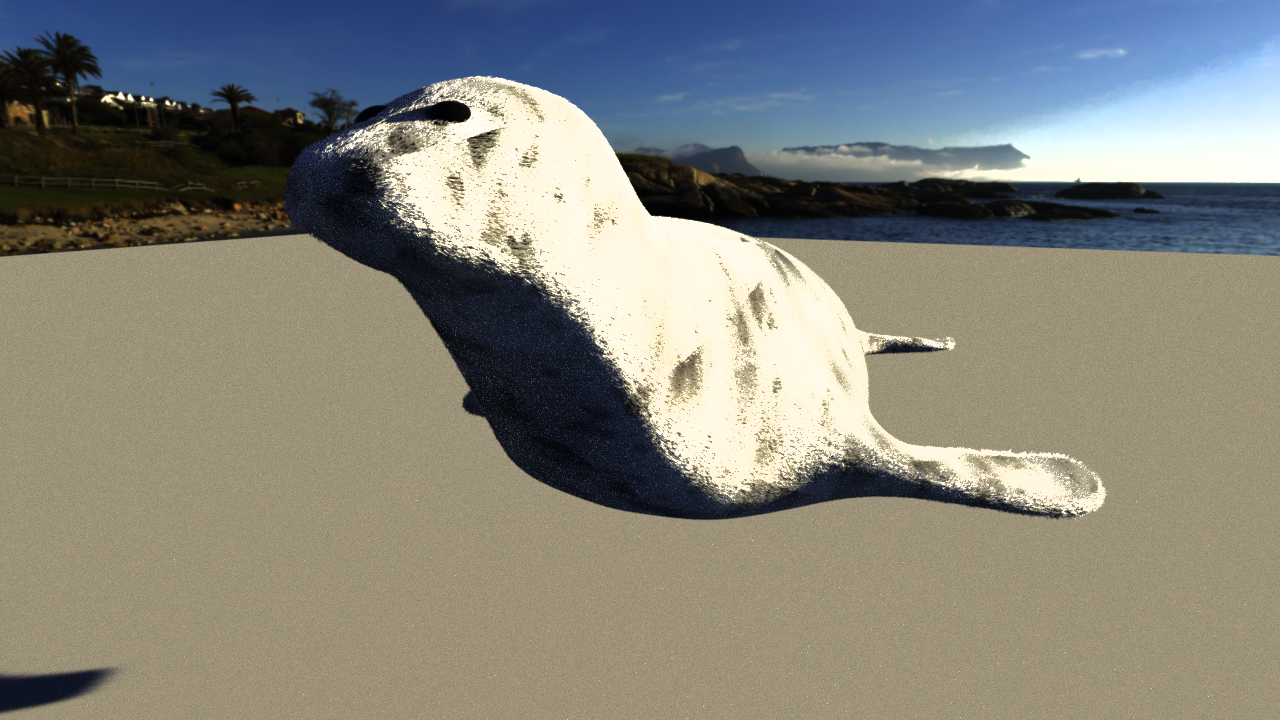
\includegraphics[width=\textwidth]{seal_dry.png}
        \caption{Dry Seal -- v59 Diffuse Fallback}
    \end{subfigure}
    \hfill
    \begin{subfigure}[b]{0.48\textwidth}
        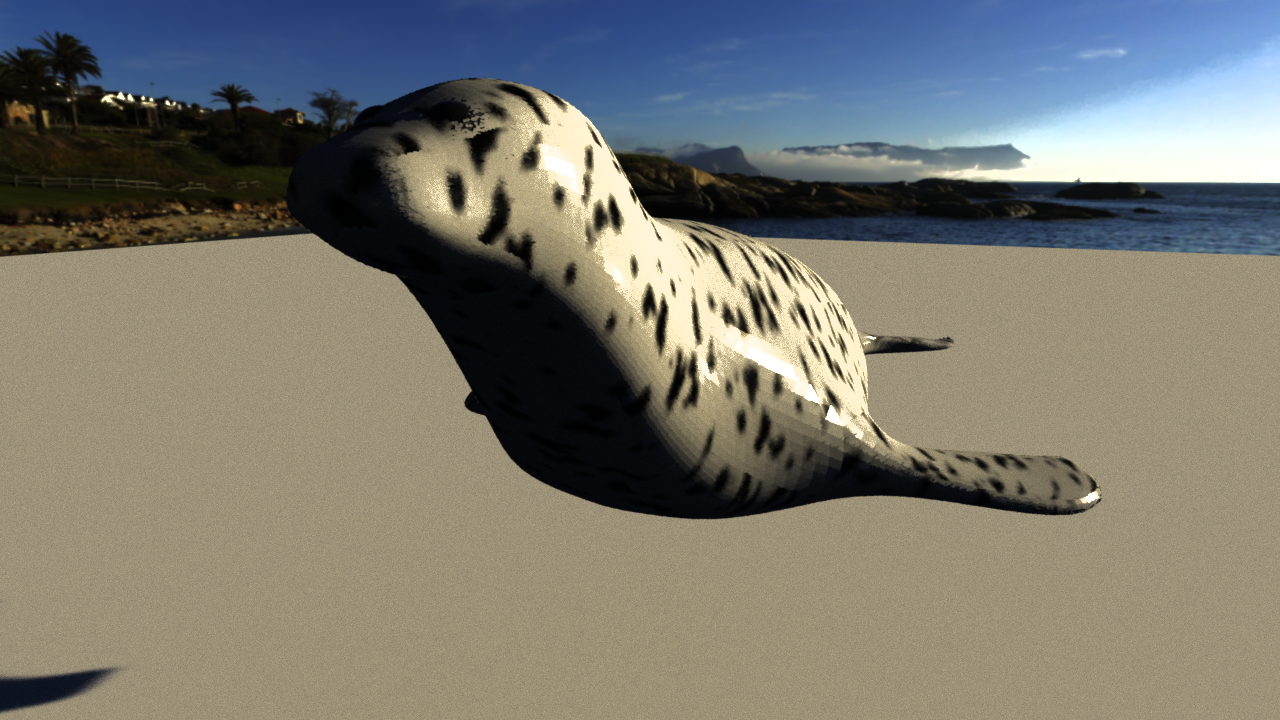
\includegraphics[width=\textwidth]{seal_wet.png}
        \caption{Wet Seal -- v42 IOR-Matched Oil Coat}
    \end{subfigure}
    \caption{Final side-by-side comparison. Both renders use \texttt{envmap scale="1.0"} and fully energy-conserving BSDFs. The dry seal shows the silver-gray base and visible dark spots; the wet seal shows the deep absorption and continuous specular sheet of the oil film.}
    \label{fig:final_comparison}
\end{figure}

\begin{table}[H]
\centering
\begin{tabular}{lll}
\toprule
\textbf{Property} & \textbf{Dry Seal} & \textbf{Wet Seal} \\
\midrule
BSDF model          & Marschner Hair BCSDF             & Oil-Coated Hair BCSDF \\
Multiple scattering & Diffuse fallback (60\% weight)   & IOR matching ($\eta_\text{eff} = 1.033$) \\
Geometry            & Upright strands, original height & Flattened to 5\%, $2\times$ radius \\
Dominant visual     & Matte, silver-gray, spots visible & Deep black, glossy oil film \\
$\sigma_a$ scale    & 0.30 (moderate)                  & 2.5 (heavy darkening) \\
Roughness $\beta_m$ & 0.40 (soft)                      & 0.03 (sharp) \\
\bottomrule
\end{tabular}
\caption{Comparison of final dry and wet seal configurations.}
\label{tab:comparison}
\end{table}

% ---------------------------------------------------------------
\section{Conclusion}
% ---------------------------------------------------------------

This project demonstrates that physically correct, artifact-free fur rendering requires solutions at multiple levels simultaneously. The three main lessons are:

\begin{enumerate}
    \item \textbf{Physics, not hacks:} Energy conservation must be maintained (scales $\leq 1.0$). When the single-scattering Marschner model loses energy in dense fur, the correct fix is a bounded diffuse fallback representing multiple scattering -- not an illegal scale multiplier or a boosted environment.
    \item \textbf{Geometry matters:} Both the specular quality (macro-normals decoupled from micro-cylinders) and the geometric deformation (flattening, clumping) are as important as the optical model for a convincing wet appearance.
    \item \textbf{Stability is not optional:} Microscopic Embree curves with HDRI lighting are a numerical minefield. A multi-level clamping hierarchy -- from BSDF/PDF ratio to the final accumulation buffer -- is necessary to keep renders clean without sacrificing legitimate highlights.
\end{enumerate}

% ---------------------------------------------------------------
\bibliographystyle{acmsiggraph}
\begin{thebibliography}{99}
\bibitem{marschner2003light}
    S.~R.~Marschner, H.~W.~Jensen, M.~Cammarano, S.~Worley, and P.~Hanrahan.
    \newblock Light scattering from human hair fibers.
    \newblock \textit{ACM Transactions on Graphics (SIGGRAPH)}, 22(3):780--791, 2003.
\bibitem{kajiya1989rendering}
    J.~T.~Kajiya and T.~L.~Kay.
    \newblock Rendering fur with three dimensional textures.
    \newblock \textit{ACM SIGGRAPH}, 23(3):271--280, 1989.
\bibitem{burley2012physically}
    B.~Burley.
    \newblock Physically-based shading at Disney.
    \newblock \textit{SIGGRAPH Physically Based Shading in Theory and Practice}, 2012.
\end{thebibliography}

\end{document}
